% Created 2022-10-29 Sat 19:03
\documentclass[9pt, b5paper]{article}
\usepackage{xeCJK}
\usepackage{minted}
\usepackage[T1]{fontenc}
\usepackage[scaled]{beraserif}
\usepackage[scaled]{berasans}
\usepackage[scaled]{beramono}
\usepackage{graphicx}
\usepackage{xcolor}
\usepackage{multirow}
\usepackage{multicol}
\usepackage{float}
\usepackage{textcomp}
\usepackage{algorithm}
\usepackage{algorithmic}
\usepackage{latexsym}
\usepackage{natbib}
\usepackage{geometry}
\geometry{left=1.2cm,right=1.2cm,top=1.5cm,bottom=1.2cm}
\newminted{common-lisp}{fontsize=\footnotesize} 
\usepackage[xetex,colorlinks=true,CJKbookmarks=true,linkcolor=blue,urlcolor=blue,menucolor=blue]{hyperref}
\author{deepwaterooo}
\date{\today}
\title{Unity Android SDK/NDK 俄罗斯方块砖3D小游戏}
\hypersetup{
  pdfkeywords={},
  pdfsubject={},
  pdfcreator={Emacs 27.1 (Org mode 8.2.7c)}}
\begin{document}

\maketitle
\tableofcontents


\section{游戏基本场景设计}
\label{sec-1}
\begin{itemize}
\item debugging game flow, 现游戏的主场景如下(看起来很丑,但它运行!!!):
\end{itemize}

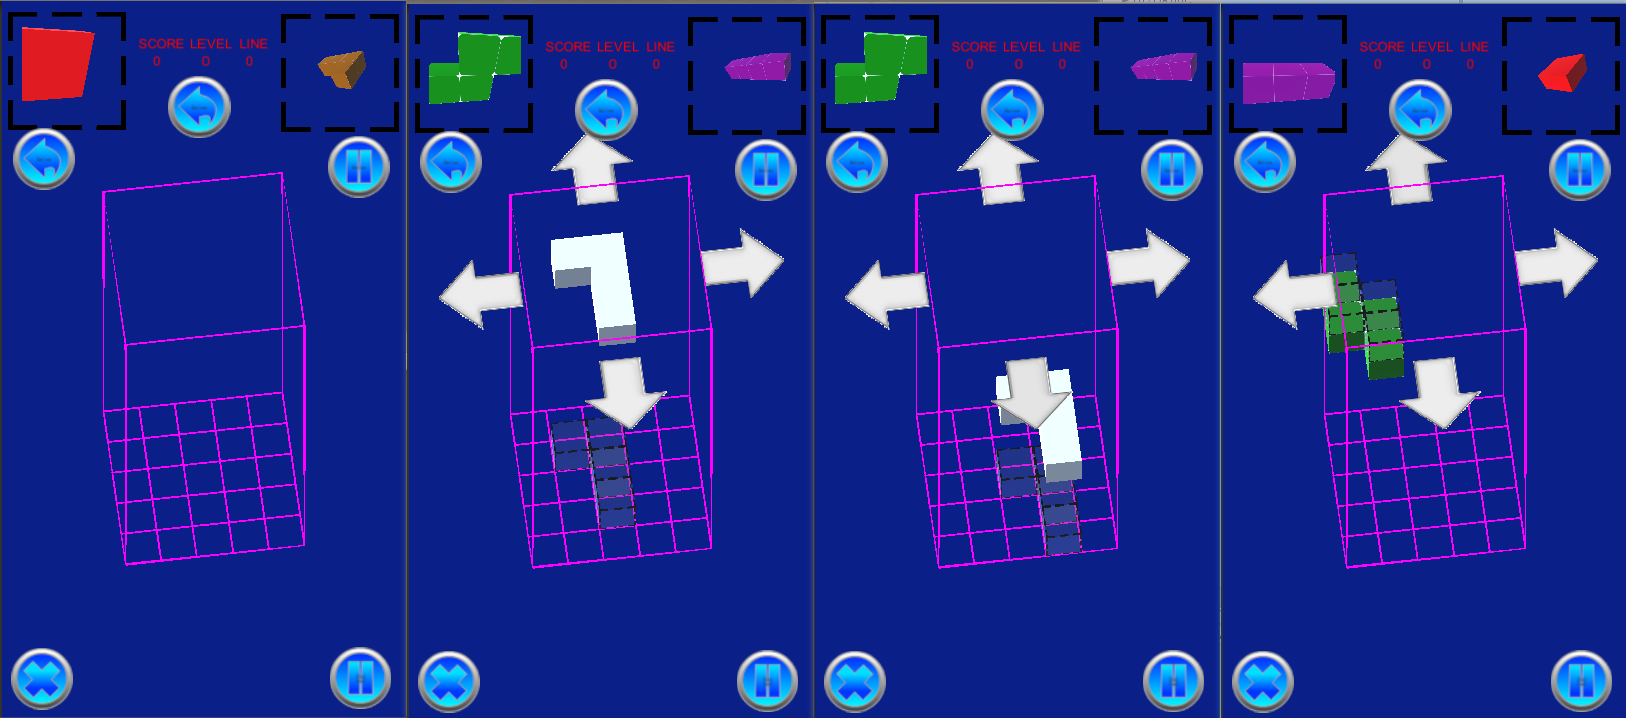
\includegraphics[width=.9\linewidth]{./pic/readme_20221029_110512.png}

\begin{itemize}
\item \textbf{TODO:}
\item AudioManager这个模块的实现暂时还没有遇到什么不适配的问题(BUG: 游戏音乐暂停后,当游戏恢复,背景音乐还没能恢复),PoolManager有不适配的问题,暂放一下(这个模块继续放在ViewManager里).接下来先把游戏里另一个主要的传导系统Evenet delegate的逻辑在热更新域里理通理顺,方便热更新程序域里有个比较好的架构
\begin{itemize}
\item \textbf{TO BE FIXED: 试了两种不同的体系:将所以点击事件与代理放热更新域与,把点击事件的触发与回调类型放主工程,热更新中只作回调,都可以做到无运行时错误,但点击回调体系还没有连通.我觉得理论知识上这块儿还有点儿欠缺,需要一两个早上把这块的理论再理解得透彻一点.会试着使至少这两个体系中的某一个运行,作为热更新里主要按钮点击回调体系的构建}
\item 我觉我的整个事件传递系统可以完全放在热更新里面来做.放在两个不同的域(把事件的定义与管理器放在主工程的坏处是:它好像建了两个不同的管理器,这会造成很多不便,希望只有一个管理器来管理所有的事件,所以可以很快放弃这个不成熟的想法)
\end{itemize}
\end{itemize}

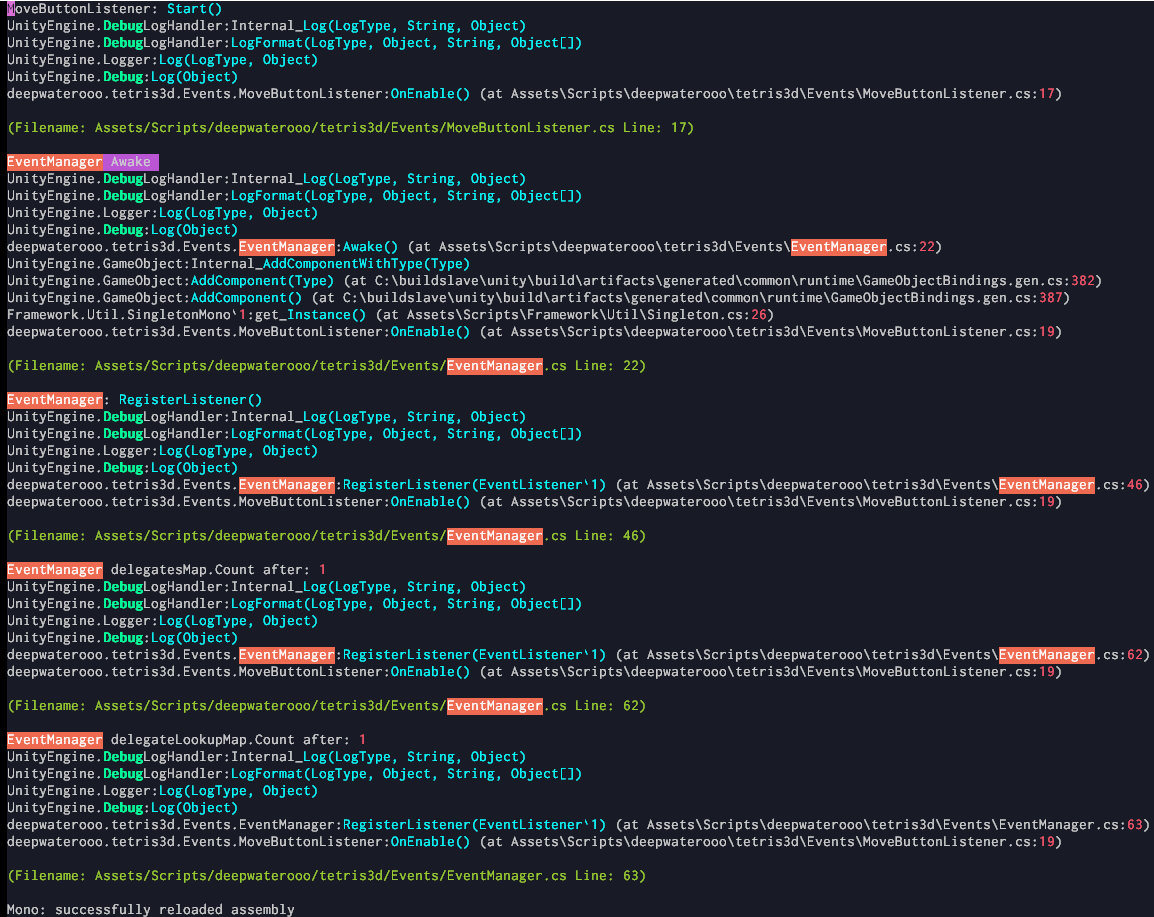
\includegraphics[width=.9\linewidth]{./pic/readme_20221029_185957.png}

\begin{itemize}
\item BUG:阴影方块砖最开始的位置还是对的,可是的后来的位置不对,会跑到方块砖的上面
\item 重要的逻辑基本都已经解决,剩下的就是把游戏的逻辑连通(今天中午吃多了,下午傍晚脑袋都不是很好用)
\item 接下来三天给自己放假远足到WSU的校园去看足球赛,不更新,周六会接着更新
\item 继续现在改好的逻辑,把游戏逻辑连起来.基本现在能够想到的比较难一点儿的全都连通了,狠开心,爱表哥,爱生活!!!
\item 昨天平移和旋转画布上的两组按钮的点击事件没有问题;可是今天UI面板上有些按钮点不通,这个点击事件的传递系统,也还需要花点时间.热更新程序域里的绝大部分按钮都是点得通可以回调的,平移组四个按钮,旋转组应该也没有问题,主游戏界面暂停按钮也可以好好工作,只是有些按钮还连不能,感觉是其它问题. (同类按钮,同一面板上的按钮,能够有一个可以运行,那么这个大的框架逻辑是通的,就不用担心了,剩余只将是细节上的小修改)
\item 现在最主要的逻辑有以上两个问题.但都能够解决.(两个基本都解决了!!!强大的debugging strategy!!! 爱表哥, 爱生活!!!)
\begin{itemize}
\item <Tetromino> <GhostTetromino> 继承自MonoBehaviour的脚本在运行时添加适配过程中出意外: instance总是空,也可以说是我的AddComponent<T>方法没有适配?这个类型的适配有点儿没有做好(这个应该是目前最重要的问题,但不是不能解决的问题)把官方DEMO中的例子好好运行好研究透彻再来试图解决自己目前遇到的问题(两个项目可以参考)
\item 我不知道现存的方案里其它人的项目是如何实现的.回到问题的本质,那就变成为最简单的办法, 便是自己实现一个计时系统,或是模拟一个每隔(比如说1秒钟,方块砖就下降一格就可以了,that's it!)这次重构想要达到的目标便是基本绝大部分的逻辑都可以热更新重构.那么只要我能够模拟每隔一秒更新一次就解决问题了,这个项目对于我来说80\%逻辑理顺,剩下的就是热更新的服务器了
\item 自己实现计时器的方法大致思路:那就分section,每个小节玩5分钟,挑战模式可以加到10分钟;每个方块砖每隔两秒下降一格;需要考虑应用的离线时间,就是游戏过程中去玩别人的应用了,再回来时间连续计算一个小节5分钟
\item 今天下午理过思路包括:
\begin{itemize}
\item 刚才没有把问题想明白:因为经过了适配,本身的UnityEngine.AddComponent<T>() UnityEngine.GetComponent<T>() 在热更新工程中的正常运行是没有问题的
\begin{itemize}
\item 出问题的特殊之处是在: Tetromini.cs GhostTetromino.cs是在热更新工程中定义的,当游戏运行,unity工程无法得知热更新工程中Tetromino.cs GhostTetromino.cs为何物
\item 上面说得不对,因为加component本身是在热更新工程中,它是知道自己工程中所定义的部件的
\end{itemize}
\item 所以得想办法把这两个类移到Unity工程中来(这个反而可能会比较繁琐,也可能逻辑不通)
\item 按照官方建议,我们是可以重置这两个方法的,让它有办法认得热更新工程中所定义的脚本(顺着这条途径把问题理顺,那么就发现别人的控件逻辑是在Unity主工程的,也就是有主工程中的MonoBehaviour系来驱动各生命周期事件,但是我的热更新控制逻辑是在热更新工程中,并没有一个默认的游戏引擎来驱动事件的自行发生)
\item 所以,没有设置好的原因,另一个是在热更新工程中,我没有哪个地方来调用UNITY工程的系统的自动运行;
\begin{itemize}
\item 前面的各种适配是适配给unity,让它认识热更新工程中的诸多类型函数等
\item 可是按照自己游戏逻辑,感觉更像是热更新工程中需要适配unity MonoBehaviour的生命周期事件 ?
\item 那么再回到上面,刚想过的
\end{itemize}
\item 所以得想办法把这两个类移到Unity工程中来(这个反而可能会比较繁琐,也可能逻辑不通)
\begin{itemize}
\item 那么这么试一下,倒还是有可能的,unity MonoBehaviour系能够自动驱动生命周期事件,引导必要时候游戏的进行 ??? 测试一下
\end{itemize}
\end{itemize}
\end{itemize}

\item 示例工程中这些劫持是,代码适配用于提供给Unity工程来加载或是获取(AddComponent<>(), GetComponent<>())热更新工程中unity所不认识的定义的类等,与自己游戏逻辑不同,不用        

\begin{itemize}
\item AudioManager,EventManager可能需要适配,就需要自己把原理都弄明白了
\item 先前的PoolManager的解决是采用ViewManager里静态管理的方法,可以如期运行,有待优化
\item 那么上面两个如果一时半会儿找不到更好的办法,就可以参照上面的方法解决
\end{itemize}
\end{itemize}

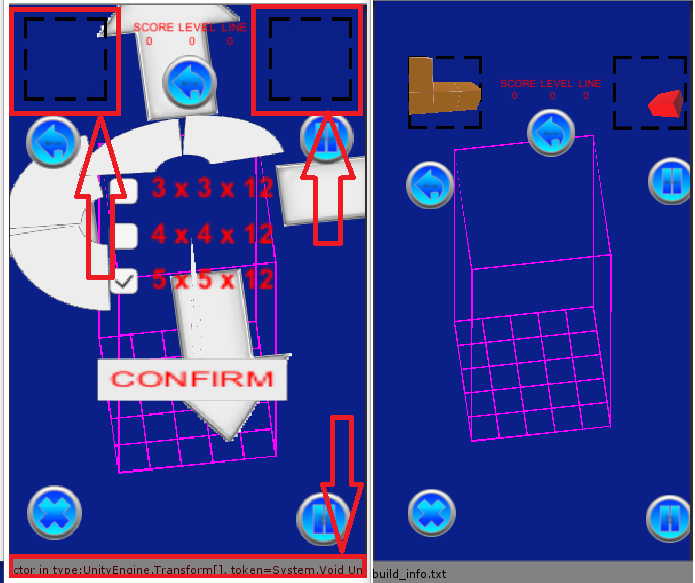
\includegraphics[width=.9\linewidth]{./pic/readme_20221020_195727.png}
\begin{itemize}
\item \textbf{已经解决了的先前的}
\item 预设都做好了,现在要将预设打资源包,并从资源包读出来供视图实例化等
\item finding the easist way to refactor yet still be able to hotfix after app installed already.
\item 现在游戏显示都没有问题了,开始debug 游戏逻辑以及功能模块等(现在只是运行了可模拟测试版的,需要在热更新程序域里将这些逻辑重构到运行出这种效果来,明天写,明天下午写?还是什么时候来写这点儿呢?)
\begin{itemize}
\item trying to link all necessary game logics and make game to run again in ILRuntime HotFix 程序域里.
\end{itemize}
\end{itemize}

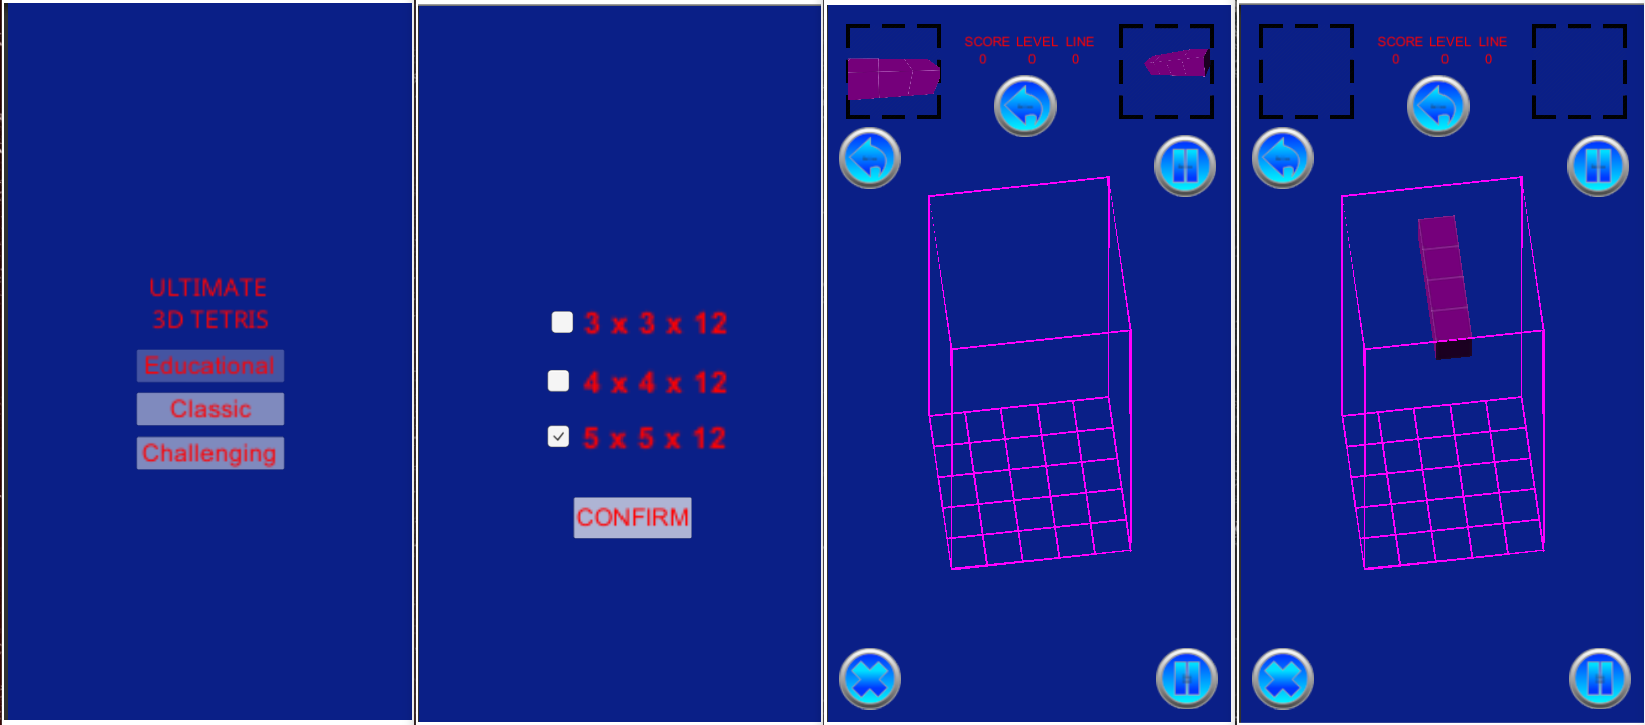
\includegraphics[width=.9\linewidth]{./pic/readme_20221022_223927.png}
\begin{itemize}
\item moveCanvas rotateCanvas上点击事件,事件系统的传递.如果上面的问题一时半会儿解决不了,可以先试图解决这个并测试一下,给上面最难的BUG一点儿网络搜索和解决问题的时间 (狠好解决)这里只是用了最基础的方法来实现,以前自己都曾实现过事件系统,现在只是测试和解决主要关键点,知道都可行可实现,会再进一步的使用适当的设计模式来优化源码
\item 两个预览方块砖的生成并画到视图上去: 现在解决这个问题
\begin{itemize}
\item 原理很简: 将两个预览放在不会出现在主相机的两个固定的位置上;再用两个不同的相机分别照在两个预览上,并分别投射到一块渲染媒介,显示在屏幕的固定投影位置上就可以了
\item 大致原理如此,但运行时存在:场景里各不同视图会被某些不确定的因素旋转某些角度,以及放大缩小位数的问题.
\item 运行时可能涉及这块投影渲染媒介的实例化(不知道目前不能很好地渲染是否是因为我打包时没有打包它?还是说因为他们出现在两个不同视图的原因呢?)
\item 就是因为如上的目前我还不太理解的不确定性,给这个游戏的unity视图显示造成一定的困难,但也不是都解决不了的,需要花时间来慢慢解决这些小问题
\end{itemize}
\item at least temporatorily passed inital running 
\begin{itemize}
\item 现两个主要的小问题:多维数组在ILRuntime热更新程序域里的适配,
\item 多维数组,稍微改动了一下就可以了,但里面还是有点儿小机关的
\begin{itemize}
\item AOT不能使用二维数组(多维数组)例如bool[,]e
\item 使用时报System.Boolean[,]::Get没有生成AOT代码
\item 改用bool[][]是OK的
\item ILRuntime Version
\item 1.6.7
\item 答案是: 需要正确生成clr绑定
\end{itemize}
\end{itemize}
\item 热更新里重新实现在的游戏主场景如下:
\end{itemize}

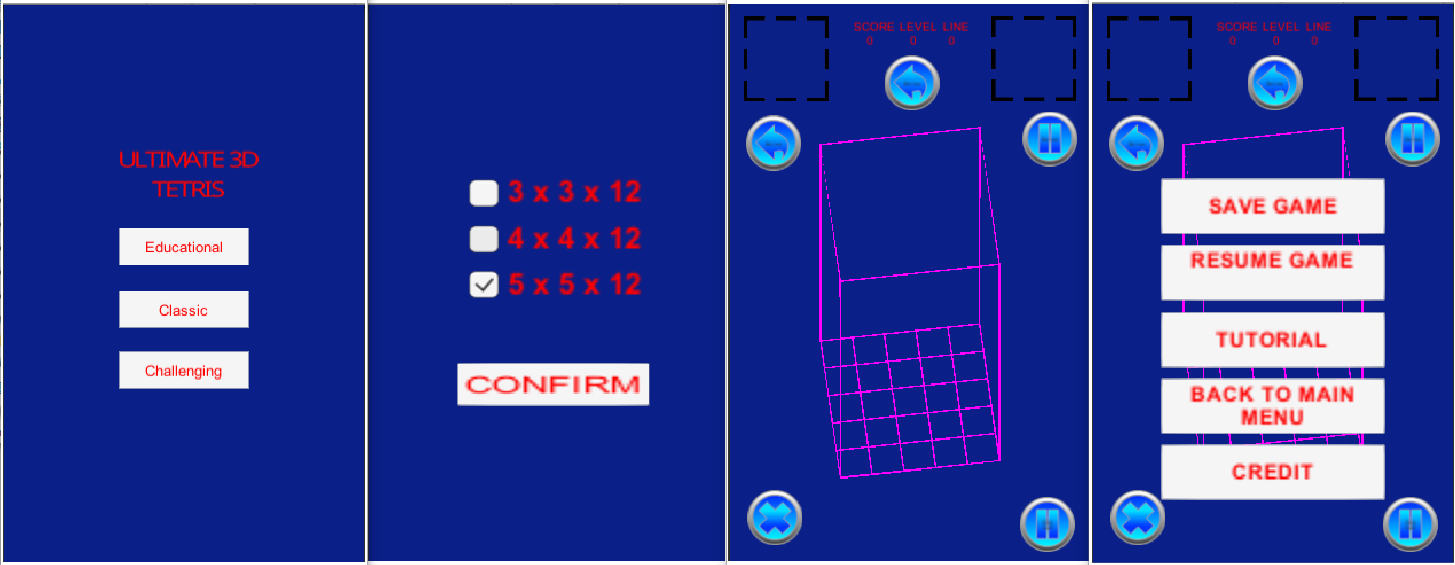
\includegraphics[width=.9\linewidth]{./pic/readme_20221011_201317.png} 
\begin{itemize}
\item 主游戏菜单与游戏过程中选择菜单: 最右为Educational has 3 choices:
\end{itemize}

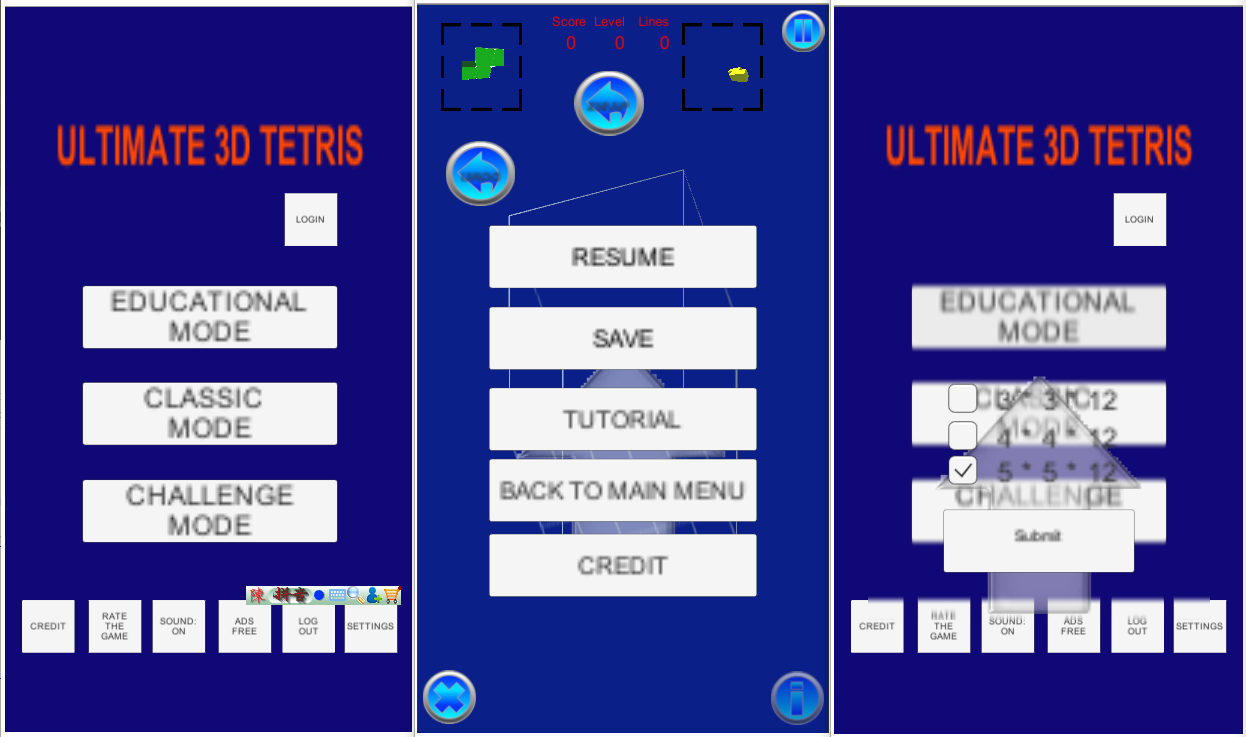
\includegraphics[width=.9\linewidth]{./pic/readme_20221007_192732.png}
\begin{itemize}
\item 启蒙模式原本是想给小盆友玩儿的,有无限撤销方块功能,和粒子消除行与列。但是这具模式有可能最终被我砍掉,相关功能改加到其它模块 
\item 启蒙模式下的由易到难三种选择:Educational mode的三种不同界面
\end{itemize}

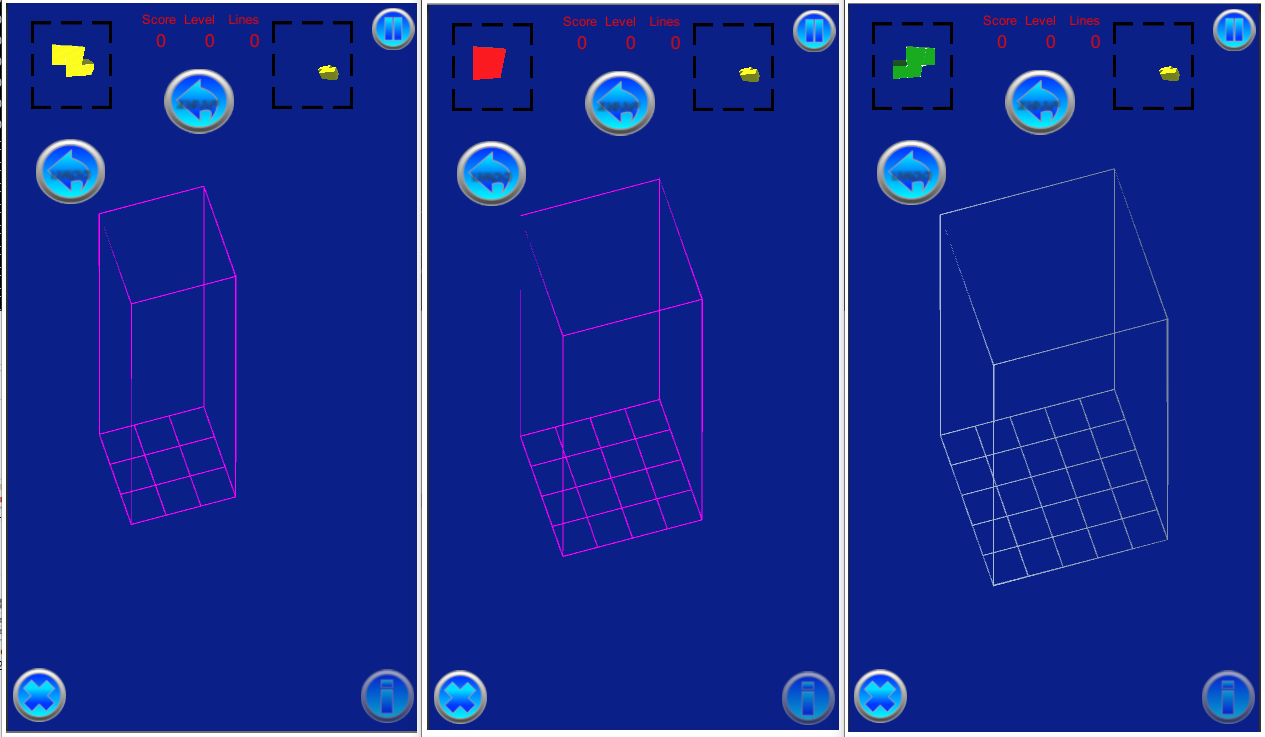
\includegraphics[width=.9\linewidth]{./pic/readme_20222007_193727.png}

\begin{itemize}
\item 传统游戏界面视图:(挑战模式下的界面丢了,到时候再补吧,或者可能只做7级,剩余热更新)
\item 两组共10个对各小方块砖方块砖平移与旋转的操纵:  \textbf{平移与旋转按钮都太丑,的摆放与位置需要优化}
\item load new game or saved games: 保存游戏数据的地址需要再改变一下,改变到应用的内部,而不是要存到什么其它的盘
\end{itemize}

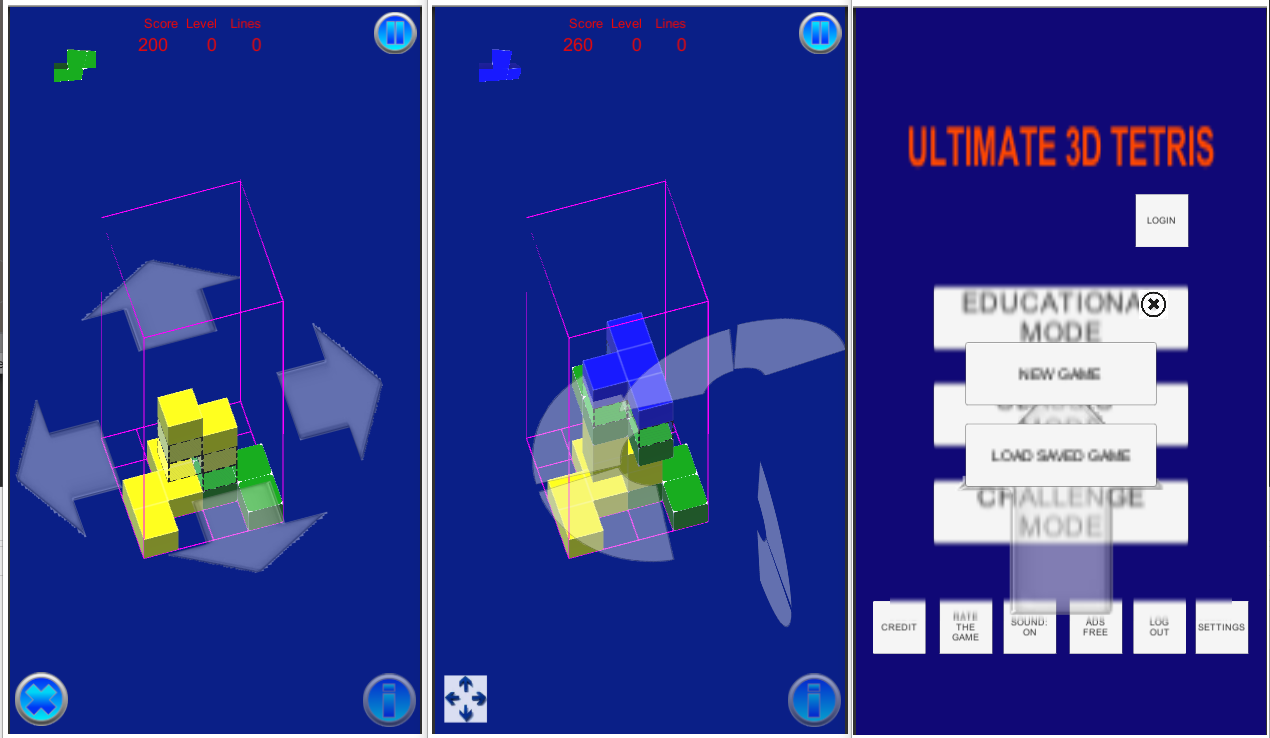
\includegraphics[width=.9\linewidth]{./pic/readme_20221007_195217.png}
\begin{itemize}
\item 现在是热更新的框架到上个周末就搭好了,这一两天忙点儿,必要的游戏场景视图基本搭配到位: 场景的搭建没有任何复杂的地方,只是相机的使用相对不够熟练,所有的都只是场景搭建基本功
\end{itemize}
m
\section{大致进展计划}
\label{sec-2}
\begin{itemize}
\item 不管是什么方法,适配原源码也好,基本也解决了现热更新程序域里的所有编译错误,现在就是解决运行游戏过程中可能会遇到的所有问题,让游戏在热更新框架下能够顺利运行起来
\begin{itemize}
\item 处理立方体与方块砖资源包的打包与读取到视图中作必要的准备,供运行时实时实例化,ViewManager.cs整合资源池
\item 必要的预设都做好了,要再理解一下从文本读取脚本资源,运行中与预设是如何结合起来生成实例的,把这部分的逻辑连通
\end{itemize}
\item 重构把代码搬过来的编译错误也比较多,就严格按照游戏的逻辑来,一步一步地添加使之运行,解决重构过程中可能会遇到的所有问题.比如现在,就先让教育模式下的两个供选择方块砖在游戏主视图加载的时候能够显示出来
\item 暂时不处理摄像机与场景相关,摄像机视角的热更新等游戏的主要逻辑完成后作为高级附加功能再添加整合模块;因为方块砖游戏中只涉及到一个场景,所以暂时不处理场景的热更新打包与加载等,使用框架但细节略过,因为场景中基本没有多的逻辑需要处理.
\item \textbf{框架搭好测试运行好了}, \textbf{必要的游戏场景资源建好了};接下来 \textbf{会侧重游戏逻辑MVVM设计模式,视图与视图数据的分离与监听通知等}
\item 要上手就来一个怎样很好的设计,对于目前来说还是相对庞大的游戏来说,可以也并不是一样容易的事.
\item 游戏几年前的实现逻辑大部分还能够回想得起来, \textbf{比较可行的办法是按照游戏的执行逻辑,在热更新程序包里先一步一步链接好,能够使游戏先运行起来,在功能模块的不断的添加过程中,一再优化这里面的数据或是热更新程序包里的游戏逻辑架构设计}
\item 现手上的资源项目没有使用View与ViewModel的数据双向传递(或者是说ViewModel部分的逻辑根本就没有或是没有实现),会再检查一遍.这里就需要仔细地去想,怎么模块化管理自己游戏中的数据(MVVM, 为什么网络上他们会用MVC或是MCP呢)
\item View和ViewModel,在创建视图的时候就自然绑定视图模型了.那么相应的视图模型就以观察某些数据(是视图观察视图模型中的数据变化--自下向上传递;视图中的按钮点击又下发更改相关数据等的逻辑,自上向下传递)
\item 搭桥: 怎么把单个视图层数据转变成为全局可访问数据,接触到过的方法有写入Settings.Global ContentProvider, 用SharedPreference写入配置文件等.这里考虑在热更新程序域里的特殊性
\item 旋转按钮的画布做得非常差(功能上相对完整,只是看起来很差),需要很有效地优化
\item 更高层级的要求是使用UniRx,但是现在还是先实现出一套可运行的逻辑才再使用UniRx的响应式编程吧\ldots{}..
\item 资源池的部分:
\item 把框架里面的root view的概念理解清楚:建立起这个概念对于应用中主要游戏场景的隐藏与显示会比较方便调控
\item 立方体与方块砖打在什么资源包里比较好,怎么打包,把他们单独打成一个包.把它们单独打一个大包,就相应的逻辑来读取这个立方体方块砖资源包<<<<<<<<<<<<<<<<<<=================
\item Mino Tetromino阴影等的预设都狠好做(会把平移与旋转视图今天上午做好,帮助推进游戏逻辑); 难的是高强偶合的游戏逻辑的模块化元件化解偶合,游戏逻辑的折解与链接
\item Unity中使用Json进行序列化与反序列化:理解,以及在方块砖项目中的使用,包括了资源打包相关的序列化与反序列化,以及游戏进展进度数据的保存与加载序列化反序列化.这里涉及到一点点儿OOD设计,从TRANSFORM到mino序列化,到方块砖序列化,到游戏进展进度数据的序列化等层层嵌套\ldots{}..
\begin{itemize}
\item 热更新重构前自己的游戏里的存储系统是使用的binaryformatter,但是现在可能把这个存储系统重构成为使用Json序列化与反序列化
\begin{itemize}
\item 前几年的理解力有限,以前力所能及地想要提高效能的办法是,比如消掉一行的时候,某个元件L只消掉了右边的短横,那么我只回收右边的短横;并且我的资源池里也缓存到了每个小立方体的级别
\item 现在重构一时半会儿还没有弄懂游戏场景的打资源包与从资源包加载初始化(因为我的游戏可以只有一个场景,其它全都只是视图的切换),没有弄透游戏里的这个元件的序列化与反序化,与自己先前的实现相比,优恶各在什么地方?如何在热更新里更为优雅地实现序列化反序列化同时还保证性能,这些问题我一边试图透过更多的视角来理解现在项目体系中的某些设计与实现,也会想要再网络搜索一下,希望尽快能够思路清晰起来
\end{itemize}
\end{itemize}
\item 为什么一部分的数据放在数据包(主要负责序列化[与反序列化]),一部分逻辑相关的放在控制包(Model, MVC vs MVP?)? 序列化与反序列化的放数据包,逻辑调控相关的放在控制包里?
\item 需要同步弄懂的是:方块砖资源池在热更新里的使用,案例学习与自己游戏逻辑的实现
\item 游戏暂时不考虑相机的动态调整与保存,只当它只有一种固定不变的设置
\item 把Unity程序域里定义的框架ILRuntime MVVM等主要模块都还理解得比较透彻了;会去深入理解热更新程序域里的数据驱动与传递,作要的research,把热更新程序域里的数据传递模块理解和设计好
\item 前段时间一直想当然天真地以为这个框架是ILRuntime + MVVM设计模式,实际上因为框架中使用了UniRx,这个框架应该更多的是MVP? 需要再好好读一下理解一下框架中的双向数据传递以及数据驱动等,把这些都弄懂理顺
\end{itemize}

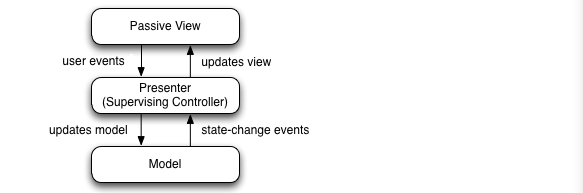
\includegraphics[width=.9\linewidth]{./pic/readme_20221012_085735.png}
\begin{itemize}
\item MVP设计模式 Model-View-(Reactive)Presenter Pattern
\item 用UniRx可以实现MVP(MVRP)设计模式。
\item 为什么应该用MVP模式而不是MVVM模式?Unity没有提供UI绑定机制,创建一个绑定层过于复杂并且会对性能造成影响。 尽管如此,视图还是需要更新。Presenters层知道view的组件并且能更新它们。虽然没有真的绑定,但Observables可以通知订阅者,功能上也差不多。这种模式叫做Reactive Presenter:
\begin{minted}[fontsize=\scriptsize,linenos=false]{csharp}
// Presenter for scene(canvas) root.
public class ReactivePresenter : MonoBehaviour {

    // Presenter is aware of its View (binded in the inspector)
    public Button MyButton;
    public Toggle MyToggle;
    
    // State-Change-Events from Model by ReactiveProperty
    Enemy enemy = new Enemy(1000);

    void Start() {
        // Rx supplies user events from Views and Models in a reactive manner 
        MyButton.OnClickAsObservable().Subscribe(_ => enemy.CurrentHp.Value -= 99);
        MyToggle.OnValueChangedAsObservable().SubscribeToInteractable(MyButton);

        // Models notify Presenters via Rx, and Presenters update their views
        enemy.CurrentHp.SubscribeToText(MyText);
        enemy.IsDead.Where(isDead => isDead == true)
            .Subscribe(_ => {
                MyToggle.interactable = MyButton.interactable = false;
            });
    }
}

// The Model. All property notify when their values change
public class Enemy {
    public ReactiveProperty<long> CurrentHp { get; private set; }
    public ReactiveProperty<bool> IsDead { get; private set; }

    public Enemy(int initialHp) {
        // Declarative Property
        CurrentHp = new ReactiveProperty<long>(initialHp);
        IsDead = CurrentHp.Select(x => x <= 0).ToReactiveProperty();
    }
}
\end{minted}
\item 视图层是一个场景scene,是Unity的hierachy定义的。展示层在Unity初始化时将视图层绑定。XxxAsObservable方法可以很容易的创建事件信号signals,没有任何开销。SubscribeToText and SubscribeToInteractable 都是简洁的类似绑定的辅助函数。虽然这些工具很简单,但是非常有用。在Unity中使用很平滑,性能很好,而且让你的代码更简洁。
\end{itemize}

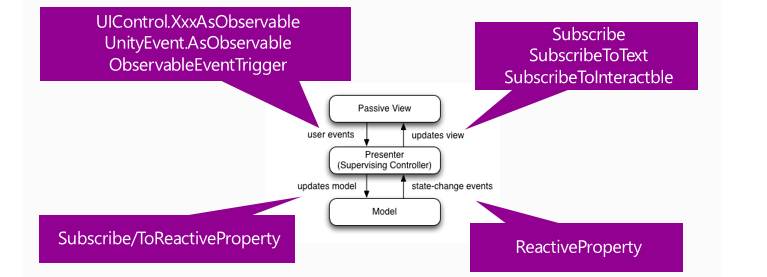
\includegraphics[width=.9\linewidth]{./pic/readme_20221012_085957.png}
\begin{itemize}
\item V -> RP -> M -> RP -> V 完全用响应式的方式连接。UniRx提供了所有的适配方法和类,不过其他的MVVM(or MV*)框架也可以使用。UniRx/ReactiveProperty只是一个简单的工具包。
\item 下面有个Rx讲给小白说的话:
\end{itemize}

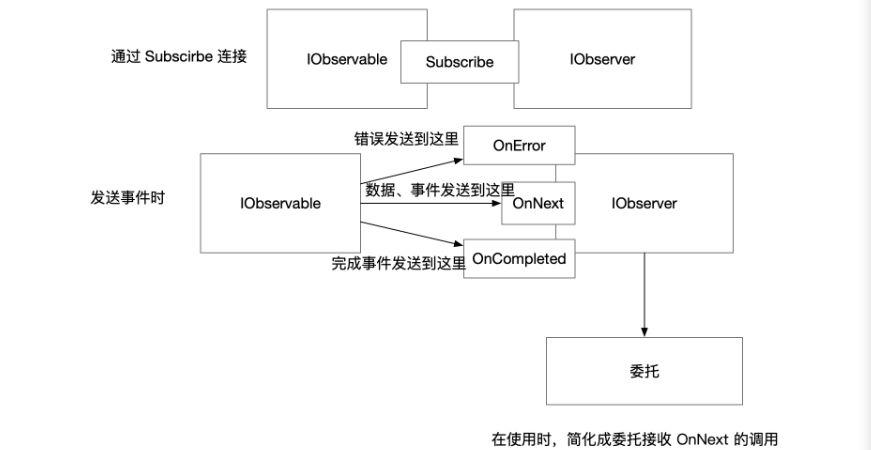
\includegraphics[width=.9\linewidth]{./pic/readme_20221012_095227.png}
\begin{itemize}
\item 今天晚上和明天就力所能力地看可以 \textbf{由现有的基本框架到明天傍晚能够实现多少基本流程}
\item 现在,进行热更新重构后,感觉 \textbf{第一要务是尽快地把现有功能都整理实现做出来,做出来是第一要务;} 丑就丑,美术和优化绝大部分实现完后才再考虑
\item 过程中纪录自己感觉需要重构或实现的点滴,需要补的知道点等;在无聊近乎麻木的重构过程中也希望能尽快地捡起需要补的知识点;希望最终整个游戏的实现流程由框架搭建测试通过,到流程由简到难都是顺畅的
\item 游戏场景里相机还需要一点儿处理(需要加一个跟踪方块砖的脚本)
\item 所有可能我还是需要把场景的热更新再理透一点儿,分场景加载应该是更有利于内存的(就是还没有使用的资源的有效的释放,但也还是看情况)

\item 以后有想法会再补这里
\end{itemize}

\section{进展过程与基本问题}
\label{sec-3}
\begin{itemize}
\item 框架基本算是已经搭建起来了(除了 \textbf{还没有热更新的服务器以} 及 \textbf{还不是很理解如何打资源包},程序代码包相对简单很多);
\item 游戏服务器打算暂时不着手处理,因为主要是 \textbf{想要深入理解ILRuntime+MVVM这个热更新框架}
\item 框架基本上算是搭起来了,但是并不是说它就能够如愿运行得狠好,现在的主要问题是热更新的程序集里还有60个左右的主要是两个不同的程序域里类型转换相关的错误需要自己一一改正.
\begin{itemize}
\item 同昨天晚上的那个错误一样,会回去检查Framework ILRuntime里的所有的错误
\item 这里也需要自己对ILRuntime的深入理解
\end{itemize}
\item 现在可以用相对较古老的版本凑合着运行起第一个视图,项目可以用相对古老的版本继续往下建下去
\item 但是我仍然希望能够自己试着去解决现存的热更新程序集里的约60个错误.这个可能会花一些时间来一一消除它们,但是值得尝试.
\end{itemize}

\section{把原理弄懂}
\label{sec-4}
\begin{itemize}
\item \textbf{热更新的服务器是自己目前的难点} ,但可以放置再决定最终是想要如何解决(用还是不用);
\item 使用unity 2017 .NET framework v3.5的热更新流程(除了场景的加载还没有去试图理解,没有太花时间在上面,因为目前的项目还不会用到)到今天下午可以完全自己实现完整了,没有任何的问题
\item Unity程序域的各种代码 + 热更新模块程序域逻辑的实现 + UI视图的各种资源打包 + Unity里热更新代码领域的资源包打包:三四个模块的基本原理弄懂弄透,基本可以达到手撕的程度了\ldots{}..
\item \textbf{框架搭建基本算是圆满完成结束;} 从今天晚上开始, \textbf{读自己原来的游戏程序代码,梳理一下接下来自己游戏玩法逻辑模块设计等,列个小计划,也需要理解触及到现有逻辑里需要重新设计或是迷补的版块} 对于自己目前不够了解或是还相对陌生的地方需要补起来
\item 热更新模块的实现:以前的设计模式和实现的功能还是比较完整的;现在更成熟一点儿(主要是理解与分析问题的能力,以及能够钻研进入解决问题的深度上比以前强太多了),需要把热更新模块补充出来;
\item ILRuntime + MVVM框架设计:两者结合,前几年的时候没能把MVVM理解透彻;ILRuntime也没有看很懂,现在基本能够看懂,大致本地的热更新流程也能建得通运行得通
\item 上次前几年主要的难点:好像是在把MVVM双向数据绑定理解得不透彻;那么这次应该就狠没有问题了,更该寻求更好的设计与解决方案; \textbf{服务器方面的知识点相对欠缺}
\item 服务器是自己现在相对的难点,但是仍然是可以暂时复制粘贴来完成热更新资源的更新的,所以还是要能够快速开发出热更新模块的游戏视图与逻辑
\item 以前被自己弄不的JAVA模式,因为现在要写CSHARP,需要把JAVA-模式给修理好,让csharp-mode代码有相对干净清洁的snippets运行环境
\item 下面有个狠好玩的图: 它描述了应用从店里下载安装后,热更新资源上载到服务器以及客户端检查更新,下载实现更新的大致过程。
\end{itemize}

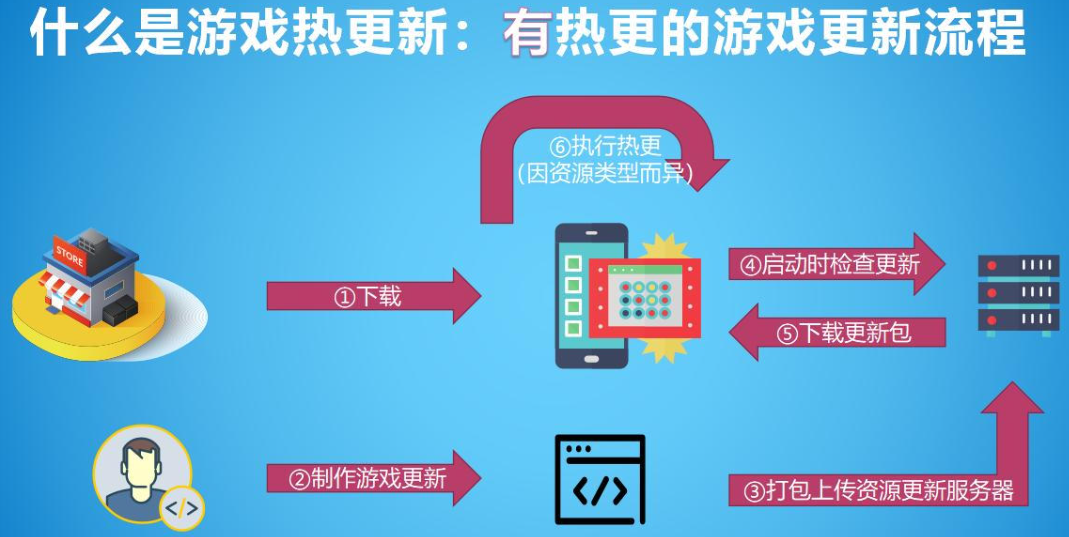
\includegraphics[width=.9\linewidth]{./pic/readme_20220930_162306.png}
- 主要是两个小项目:
\begin{itemize}
\item 资源包的准备:热更新分程序热更新和资源的热更新;那么现在的项目就是资源的热更新是分成了两个小项目来实现资源热更新资源包的自动打包(分场景打包和其它资源打包);程序热更新因为主要是更新视图,游戏的所有基本逻辑主程序都运行在热更新程序包下,所以三个小项目便可以实现所有资源(是指包括资源和程序)的自动打包为可上载热更新服务器的程序包。(三个小项目看起来是最简单的,但是全部实现出来可能还是工作量最大的)

\item 服务器层的相对理解:应该是需要一个好用的第三方程序,或是合适好有物服务器来提供必要的资源包上载到服务器;服务器层可能还需要根据不同的应用平台(IOS安卓等)来进行一定的配置,以及必要的压力测试保证相对大量用户的情况下可以正常上载下载运行(后一步暂不考虑)
\item 客户端:对于不同的客户端应用平台,游戏运行时的资源包MD5比对的原理要再熟悉一下
\item 我觉得我该考虑尽快至少建个本地服务器了
\item 性能优化:另外是对其实高级开发的越来越熟悉,希望应用的性能表现,尤其是渲染性能与速度等、这些更为高级和深入的特性成为这次二次开发的重点。

\item 现在是把自己几年前的写的游戏全忘记了,需要回去把自己的源码找出来,再读一读熟悉一下自己的源码,了解当时设计的估缺点,由此改进更将
\end{itemize}

\section{几种不同热更新模式的探讨}
\label{sec-5}
\subsection{HybridCLR——划时代的Unity原生C\#热更新技术: IL2CPP与热更新}
\label{sec-5-1}

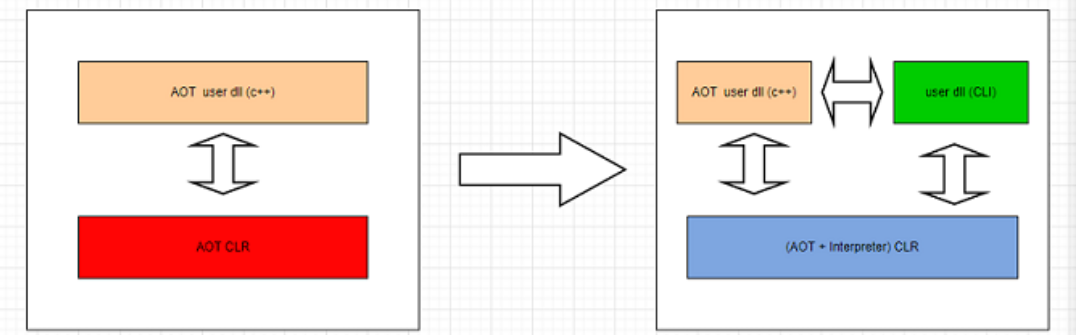
\includegraphics[width=.9\linewidth]{./pic/readme_20220930_082537.png}

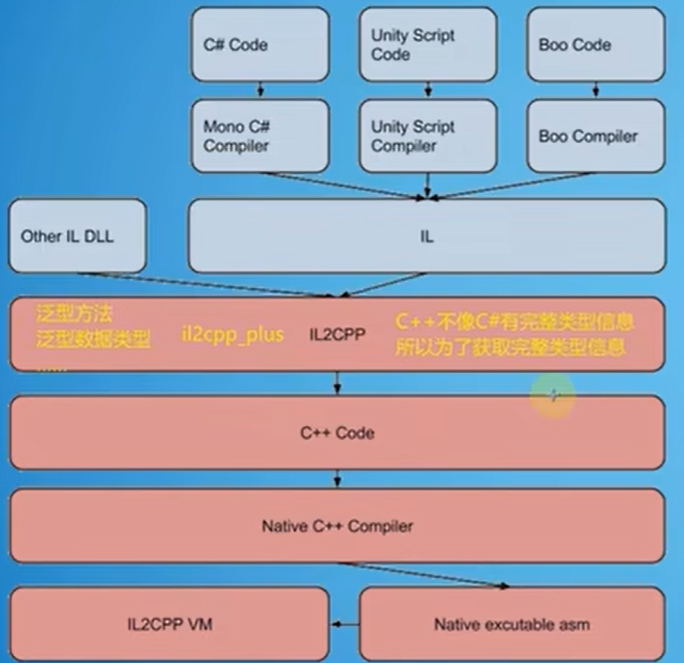
\includegraphics[width=.9\linewidth]{./pic/readme_20220930_165543.png}
很不幸,不像Mono有Hybrid mode execUtion,可支持动态加载DLL。IL2CPP是一个纯静态的AOT运行时,不支持运行时加载DLL,因此不支持热更新。
目前unity平台的主流热更新方案xLUa、ILRUntime之类都是引入一个第三方VM(VirtUal Machine),在VM中解释执行代码,来实现热更新。这里我们只分析使用C\#为开发语言的热更新方案。这些热更新方案的VM与IL2CPP是独立的,意味着它们的元数据系统是不相通的,在热更新里新增一个类型是无法被IL2CPP所识别的(例如,通过System.Activator.CreateInstance是不可能创建出这个热更新类型的实例),这种看起来像,但实际上又不是的伪CLR虚拟机,在与IL2CPP这种复杂的CLR运行时交互时,会产生极大量的兼容性问题,另外还有严重的性能问题。
一个大胆的想法是,是否有可能对IL2CPP运行时进行扩充,添加Interpreter模块,进而实现Mono hybrid mode execUtion这样机制?这样一来就能彻底支持热更新,并且兼容性极佳。对开发者来说,除了解释模式运行的部分执行得比较慢,其他方面跟标准的运行时没有区别。
对IL2CPP加以了解并且深思熟虑后的答案是——确实是可行的!具体分析参见第二节《关于HybridCLR可行性的思维实验》 。这个想法诞生了HybridCLR,unity平台第一个支持iOS的跨平台原生C\#热更新方案!
\begin{itemize}
\item 现在也简单地理解一下这个方案最简单原始案例实现的基本原理,若有兴趣,就可以再深入地探讨一下
\end{itemize}


\section{环境弄得比较好的包括:}
\label{sec-6}
\begin{itemize}
\item 电脑的配置有限,文件稍微大一点儿的时候已经不太好处理了;所以不得不分割成多个小文件
\item 几年过去了,ILRuntime已经不是最新最前沿的热更新技术,成为别人更新技术的一个子模块,所以还是自己再搜索找一下有没有更方便的热更新实现方法(若是不得,我就在自己游戏里实现 ILRuntime + MVVM实现视图等的更新)
\end{itemize}
- 这一两天作必要的文献研究,确定哪个大的模块版块需要实现或是修改优化,列个大致计划,把它们一一完成;希望截止这个周末周六周日能够把这个部分确定得相对精确
\begin{itemize}
\item 小笔记本电脑太慢了,会回家再读其它模块的源码,理解透彻。爱表哥,爱生活!!
\item 输入法的搭建:终于用到了自己之前用过的好用的输入法
\item 这两天开车疲累,最迟明天中午会去南湾找房间出租,尽快解决搬家的问题;昨天晚上回来得太晚了,一路辛苦,路上只差睡着,回到家里补觉补了好多个小时。
\item 小电脑,笔记本电脑里的游戏环境搭建,今天下午去图书馆里弄(今天下午去图书馆里把需要借助快速网络来完成的事情都搭建好;家里被恶房东故意整了个腾腾慢的网,故意阻碍别人的发展,谁还愿意再这样的环境中继续住下去呢?!!!)
\end{itemize}
- 能够把程序源码读得比较懂,也并不代表把所有相关的原理就全部弄懂了;不是说还有多在的挑战,而是说要不断寻找更为有效的学习方法,快速掌握所有涉及到的相关原理;在理解得更为深入掌握了基本原理的基础上再去读源码,会不会更为有效事半功倍呢?这是一颗永远不屈服的心,爱表哥,爱生活!!!
\section{ILRuntime 库的系统再深入理解}
\label{sec-7}
\subsection{ILRuntime基本原理}
\label{sec-7-1}
\begin{itemize}
\item ILRuntime借助Mono.Cecil库来读取DLL的PE信息,以及当中类型的所有信息,最终得到方法的IL汇编码,然后通过内置的IL解译执行虚拟机来执行DLL中的代码。IL解释器代码在ILIntepreter.cs,通过Opcode来逐语句执行机器码,解释器的代码有四千多行。
\end{itemize}

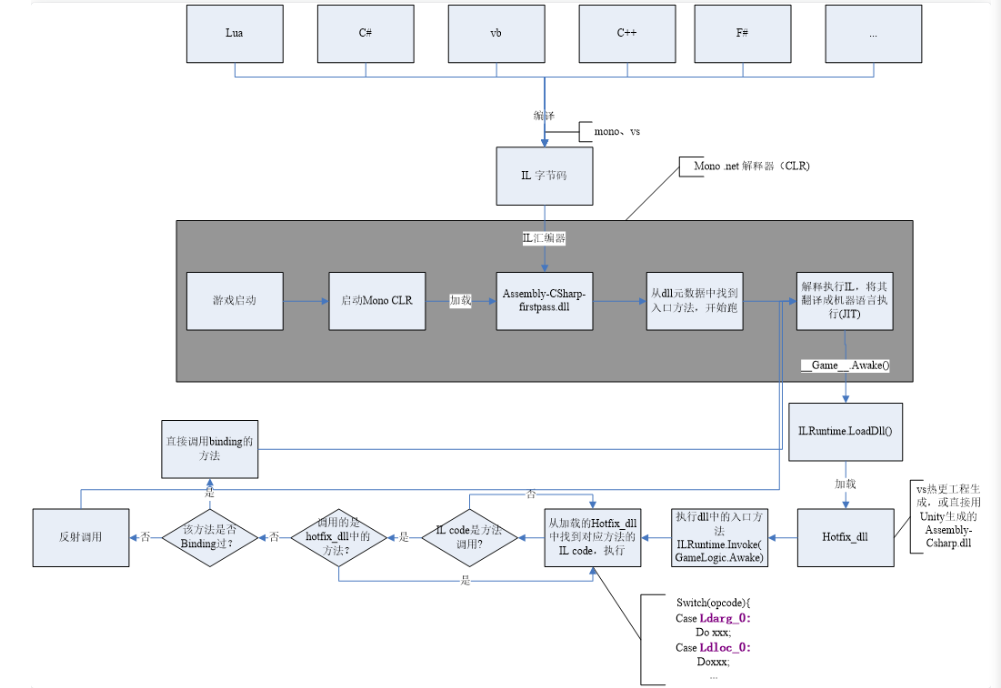
\includegraphics[width=.9\linewidth]{./pic/readme_20220926_094936.png}

\subsection{ILRuntime热更流程}
\label{sec-7-2}

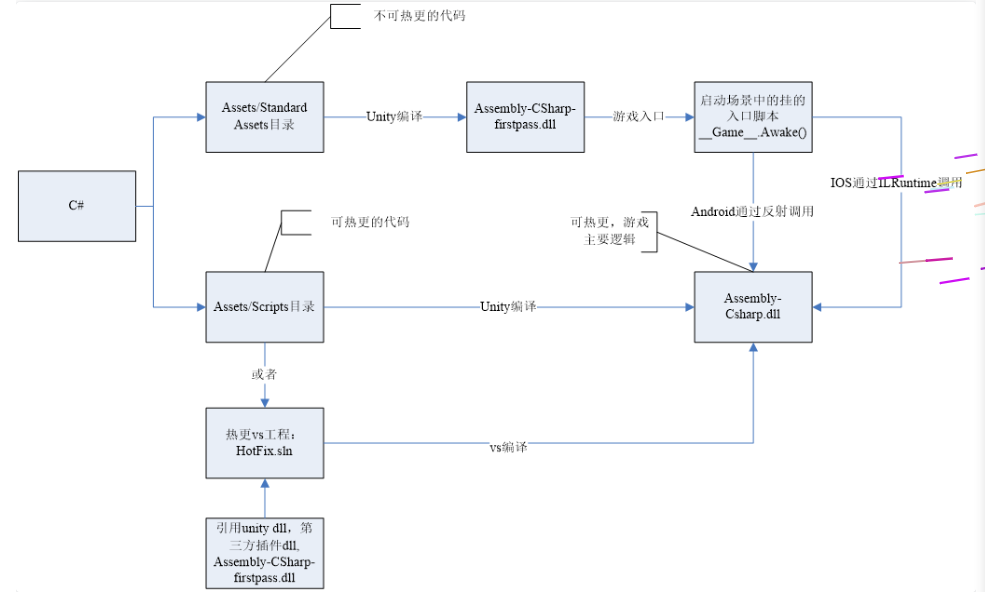
\includegraphics[width=.9\linewidth]{./pic/readme_20220926_095022.png}
\subsection{ILRuntime主要限制}
\label{sec-7-3}

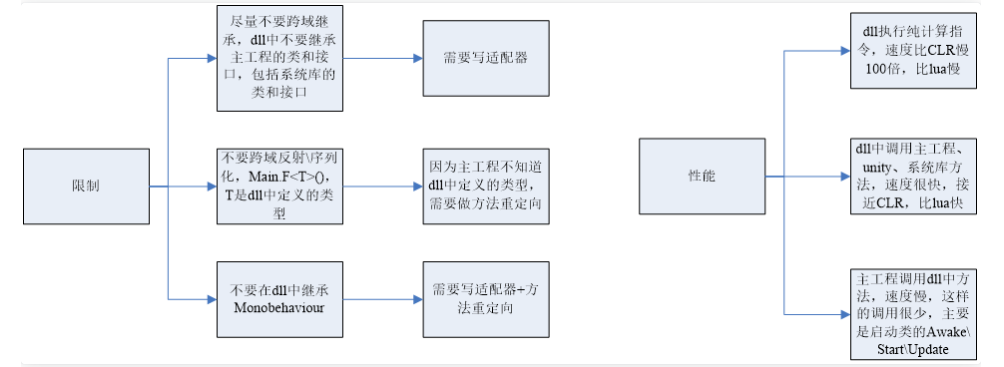
\includegraphics[width=.9\linewidth]{./pic/readme_20220926_095555.png}
\begin{itemize}
\item \textbf{委托适配器(DelegateAdapter)} :将委托实例传出给ILRuntime外部使用,将其转换成CLR委托实例。
\end{itemize}
由于IL2CPP之类的AOT编译技术无法在运行时生成新的类型,所以在创建委托实例的时候ILRuntime选择了显式注册的方式,以保证问题不被隐藏到上线后才发现。
\begin{minted}[fontsize=\scriptsize,linenos=false]{csharp}
//同一参数组合只需要注册一次
delegate void SomeDelegate(int a, float b);
Action<int, float> act;
//注册,不带返回值,最多支持五个参数传入
appDomain.DelegateManager.RegisterMethodDelegate<int, float>();

//注册,带参数返回值,最后一个参数为返回值,最多支持四个参数传入
delegate bool SomeFunction(int a, float b);
Func<int, float, bool> act;
\end{minted}
\begin{itemize}
\item \textbf{委托转换器RegisterDelegateConvertor} :需要将一个不是Action或者Func类型的委托实例传到ILRuntime外部使用,需要写委托适配器和委托转换器。委托转换器将Action和Func转换成你真正需要的那个委托类型
\end{itemize}
\begin{minted}[fontsize=\scriptsize,linenos=false]{csharp}
app.DelegateManager.RegisterDelegateConvertor<SomeFunction>((action) =>
{
    return new SomeFunction((a, b) =>
    {
       return ((Func<int, float, bool>)action)(a, b);
    });
});
\end{minted}
\begin{itemize}
\item 为了避免不必要的麻烦,以及后期热更出现问题,建议: 1、尽量避免不必要的跨域委托调用 2、尽量使用Action以及Func委托类型
\item \textbf{CLR重定向:} ILRuntime为了解决外部调用内部接口的问题,引入了CLR重定向机制。 原理就是当IL解译器发现需要调用某个指定CLR方法时,将实际调用重定向到另外一个方法进行挟持,再在这个方法中对ILRuntime的反射的用法进行处理
\item 从代码中可以看出重定向的工作是把方法挟持下来后装到ILIntepreter的解释器里面实例化
\item 不带返回值的重定向:
\end{itemize}
\begin{minted}[fontsize=\scriptsize,linenos=false]{csharp}
public static StackObject* CreateInstance(ILIntepreter intp, StackObject* esp,
                                          List<object> mStack, CLRMethod method, bool isNewObj) {
    // 获取泛型参数<T>的实际类型
    IType[] genericArguments = method.GenericArguments;
    if (genericArguments != null && genericArguments.Length == 1) {
        var t = genericArguments[0];
        if (t is ILType) { // 如果T是热更DLL里的类型 
            // 通过ILRuntime的接口来创建实例
            return ILIntepreter.PushObject(esp, mStack, ((ILType)t).Instantiate());
        } else // 通过系统反射接口创建实例
            return ILIntepreter.PushObject(esp, mStack, Activator.CreateInstance(t.TypeForCLR));
    } else
        throw new EntryPointNotFoundException();
}
// 注册
foreach (var i in typeof(System.Activator).GetMethods()) {
    // 找到名字为CreateInstance,并且是泛型方法的方法定义
    if (i.Name == "CreateInstance" && i.IsGenericMethodDefinition) {
        // RegisterCLRMethodRedirection:通过redirectMap存储键值对MethodBase-CLRRedirectionDelegate,如果i不为空且redirectMap中没有传入的MethodBase(即下方的i)则存储redirectMap[i] = CreateInstance。所以如此看来注册行为就是把键值对存储到redirectMap的过程
        appdomain.RegisterCLRMethodRedirection(i, CreateInstance);
    }
}
\end{minted}
\begin{itemize}
\item 带返回值方法的重定向
\end{itemize}
\begin{minted}[fontsize=\scriptsize,linenos=false]{csharp}
public unsafe static StackObject* DLog(ILIntepreter __intp, StackObject* __esp,
                                       List<object> __mStack, CLRMethod __method, bool isNewObj)  {
    ILRuntime.Runtime.Enviorment.AppDomain __domain = __intp.AppDomain;
    StackObject* ptr_of_this_method;
    // 只有一个参数,所以返回指针就是当前栈指针ESP - 1
    StackObject* __ret = ILIntepreter.Minus(__esp, 1);
    // 第一个参数为ESP -1, 第二个参数为ESP - 2,以此类推
    ptr_of_this_method = ILIntepreter.Minus(__esp, 1);
    // 获取参数message的值
    object message = StackObject.ToObject(ptr_of_this_method, __domain, __mStack);
    // 需要清理堆栈
    __intp.Free(ptr_of_this_method);
    // 如果参数类型是基础类型,例如int,可以直接通过int param = ptr_of_this_method->Value获取值,
    // 关于具体原理和其他基础类型如何获取,请参考ILRuntime实现原理的文档。
            
    // 通过ILRuntime的Debug接口获取调用热更DLL的堆栈
    string stackTrace = __domain.DebugService.GetStackTrance(__intp);
    Debug.Log(string.Format("{0}\n{1}", format, stackTrace));
    return __ret;
}
\end{minted}
\begin{itemize}
\item \textbf{LitJson集成}: Json序列化是开发中非常经常需要用到的功能,考虑到其通用性,因此ILRuntime对LitJson这个序列化库进行了集成
\end{itemize}
\begin{minted}[fontsize=\scriptsize,linenos=false]{csharp}
//对LitJson进行注册,需要在注册CLR绑定之前
LitJson.JsonMapper.RegisterILRuntimeCLRRedirection(appdomain);
//LitJson使用
//将一个对象转换成json字符串
string json = JsonMapper.ToJson(obj);
//json字符串反序列化成对象
JsonTestClass obj = JsonMapper.ToObject<JsonTestClass>(json);
\end{minted}
\begin{itemize}
\item \textbf{ILRuntime的性能优化}
\begin{itemize}
\item 值类型优化:使用ILRuntime外部定义的值类型(例如UnityEngine.Vector3)在默认情况下会造成额外的装箱拆箱开销。ILRuntime在1.3.0版中增加了值类型绑定(ValueTypeBinding)机制,通过对这些值类型添加绑定器,可以大幅增加值类型的执行效率,以及避免GC Alloc内存分配。
\item 大规模数值计算:如果在热更内需要进行大规模数值计算,则可以开启ILRuntime在2.0版中加入的寄存器模式来进行优化
\item 避免使用foreach:尽量避免使用foreach,会不可避免地产生GC。而for循环不会。
\item 加载dll并在逻辑后处理进行简单调用
\item 整个文件流程:创建IEnumerator并运行->用文件流判断并读入dll和pdb->尝试加载程序集dll->(如果加载成功)初始化脚本引擎(InitializeILRuntime())->执行脚本引擎加载后的逻辑处理(OnHotFixLoaded())->程序销毁(在OnDestoy中关闭dll和pdb的文件流)
\item MemoryStream:为系统提供流式读写。MemoryStream类封装一个字节数组,在构造实例时可以使用一个字节数组作为参数,但是数组的长度无法调整。使用默认无参数构造函数创建实例,可以使用Write方法写入,随着字节数据的写入,数组的大小自动调整。 参考博客:传送门
\item appdomain.LoadAssembly:将需要热更的dll加载到解释器中。第一个填入dll以及pdb,这里的pdb应该是dll对应的一些标志符号。 后面的ILRuntime.Mono.Cecil.Pdb.PdbReaderProvider()是动态修改程序集,它的作用是给ILRuntime.Mono.Cecil.Pdb.PdbReaderProvider()里的GetSymbolReader)(传入两个参数,一个是通过转化后的ModuleDefinition.ReadModule(stream(即dll))模块定义,以及原来的symbol(即pdb) GetSymbolReader主要的作用是检测其中的一些符号和标志是否为空,不为空的话就进行读取操作。 (这些内容都是ILRuntime中的文件来完成)
\end{itemize}
\item Unity MonoBehaviour lifecycle methods callback execute orders:
\item 还有一个看起来不怎么清楚的,将就凑合着看一下:这几个图因为文件地址错误丢了,改天再补一下
\item IL热更优点:
\begin{itemize}
\item 1、无缝访问C\#工程的现成代码,无需额外抽象脚本API
\item 2、直接使用VS2015进行开发,ILRuntime的解译引擎支持.Net 4.6编译的DLL
\item 3、执行效率是L\#的10-20倍
\item 4、 \textbf{选择性的CLR绑定使跨域调用更快速,绑定后跨域调用的性能能达到slua的2倍左右(从脚本调用GameObject之类的接口)}
\item 5、支持跨域继承(代码里的完美学演示)
\item 6、完整的泛型支持(代码里的完美学演示)
\item 7、拥有Visual Studio的调试插件,可以实现真机源码级调试。支持Visual Studio 2015 Update3 以及Visual Studio 2017和Visual Studio 2019
\item 8、最新的2.0版引入的寄存器模式将数学运算性能进行了大幅优化
\end{itemize}
\end{itemize}

\subsection{ILRuntime启动调试}
\label{sec-7-4}
\begin{itemize}
\item ILRuntime建议全局只创建一个AppDomain,在函数入口添加代码启动调试服务
\end{itemize}
\begin{minted}[fontsize=\scriptsize,linenos=false]{csharp}
appdomain.DebugService.StartDebugService(56000)
\end{minted}
\begin{itemize}
\item 运行主工程(Unity工程)
\item 在热更的VS工程中 点击 - 调试 - 附加到ILRuntime调试,注意使用一样的端口
\item 如果使用VS2015的话需要Visual Studio 2015 Update3以上版本
\end{itemize}
\subsection{线上项目和资料}
\label{sec-7-5}
\begin{itemize}
\item 掌趣很多项目都是使用ILRuntime开发,并上线运营,比如:真红之刃,境·界 灵压对决,全民奇迹2,龙族世界,热血足球
\item 初音未来:梦幻歌姬 使用补丁方式:\url{https://github.com/wuxiongbin/XIL}
\item 本文流程图摘自:ILRuntime的QQ群的《ILRuntime热更框架.docx》(by a 704757217)
\item Unity实现c\#热更新方案探究(三): \url{https://zhuanlan.zhihu.com/p/37375372}
\end{itemize}
\section{remember necessary positoins}
\label{sec-8}

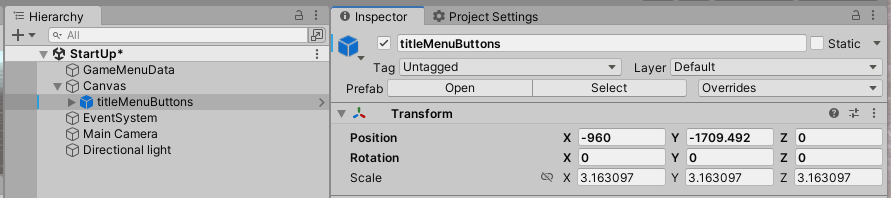
\includegraphics[width=.9\linewidth]{./pic/readme_20220930_204953.png}



\section{ILRuntime的研究}
\label{sec-9}
\begin{itemize}
\item 借助网络上别人源码分析的步骤,自己(大项目中,以前的小项目源码内容大多已经狠熟悉的小项目里找找源码的不算)找一找学习一下追溯源码的过程,去理解整个过程的关键步骤与原理、
\item \url{https://www.igiven.com/unity-2019-09-02-ilruntime/}
\end{itemize}
\subsection{工程运行的入口}
\label{sec-9-1}
\subsubsection{HotFixILRunTime}
\label{sec-9-1-1}
\begin{minted}[fontsize=\scriptsize,linenos=false]{csharp}
public class HotFixILRunTime : SingletonMono<HotFixILRunTime>, IHotFixMain {
    public static ILRuntime.Runtime.Enviorment.AppDomain appDomain;
    void Start() {
        appDomain = new ILRuntime.Runtime.Enviorment.AppDomain(); // <<<<<<<<<< 
#if UNITY_EDITOR
        appDomain.UnityMainThreadID = System.Threading.Thread.CurrentThread.ManagedThreadId;
#endif
        TextAsset dllAsset = ResourceConstant.Loader.LoadAsset<TextAsset>("HotFix.dll", "HotFix.dll");
        var msDll = new System.IO.MemoryStream(dllAsset.bytes);
        if (GameApplication.Instance.usePDB) {
            ResourceConstant.Loader.LoadAssetAsyn<TextAsset>("HotFix.pdb", "HotFix.pdb", (pdbAsset) => {
                var msPdb = new System.IO.MemoryStream(pdbAsset.bytes);
                appDomain.LoadAssembly(msDll, msPdb, new Mono.Cecil.Mdb.MdbReaderProvider()); // <<<<<<<<<<<<<<<<<<<< 
                StartApplication();
            }, EAssetBundleUnloadLevel.ChangeSceneOver);
        } else {
            appDomain.LoadAssembly(msDll, null, new Mono.Cecil.Mdb.MdbReaderProvider());
            StartApplication();
        }
    }
}
\end{minted}
\begin{itemize}
\item unity工程在执行的时候,会构建一个默认的appDomain,Assembly.Load,其实就是在这个程序域上加载Dll,所以相关的实质和前面一个部分相差不大,这就是c\#热更新在unity中的应用(IOS不包括)。
\end{itemize}
\subsubsection{LoadAssembly(System.IO.Stream stream, System.IO.Stream symbol, ISymbolReaderProvider symbolReader)}
\label{sec-9-1-2}
\begin{itemize}
\item 基于WWW的方式加载AssetBundle或者DLL/PDB后,接下来是将其封入到MemoryStream中,将dll和pdb的bytes都存入到内存流中后,执行其内部实现的LoadAssembly方法。
\end{itemize}
\begin{minted}[fontsize=\scriptsize,linenos=false]{csharp}
// 从流加载Assembly,以及symbol符号文件(pdb)
// <param name="stream">Assembly Stream</param>
// <param name="symbol">symbol Stream</param>
// <param name="symbolReader">symbol 读取器</param>
public void LoadAssembly(System.IO.Stream stream, System.IO.Stream symbol, ISymbolReaderProvider symbolReader) {

    var module = ModuleDefinition.ReadModule(stream); //从MONO中加载模块 // <<<<<<<<<<<<<<<<<<<< 

    if (symbolReader != null && symbol != null)  
        module.ReadSymbols(symbolReader.GetSymbolReader(module, symbol)); //加载符号表

    if (module.HasAssemblyReferences) { //如果此模块引用了其他模块 
        foreach (var ar in module.AssemblyReferences) {
            /*if (moduleref.Contains(ar.Name) == false)
              moduleref.Add(ar.Name);
              if (moduleref.Contains(ar.FullName) == false)
              moduleref.Add(ar.FullName);*/
        }
    }
    if (module.HasTypes) {
        List<ILType> types = new List<ILType>();
        foreach (var t in module.GetTypes()) { //获取所有此模块定义的类型 
            ILType type = new ILType(t, this);
            mapType[t.FullName] = type;
            types.Add(type);
        }
    }
    if (voidType == null) {
        voidType = GetType("System.Void");
        intType = GetType("System.Int32");
        longType = GetType("System.Int64");
        boolType = GetType("System.Boolean");
        floatType = GetType("System.Single");
        doubleType = GetType("System.Double");
        objectType = GetType("System.Object");
    }
    module.AssemblyResolver.ResolveFailure += AssemblyResolver_ResolveFailure;
#if DEBUG
    debugService.NotifyModuleLoaded(module.Name);
#endif
}
\end{minted}
\subsubsection{ReadModule(stream)}
\label{sec-9-1-3}
\begin{minted}[fontsize=\scriptsize,linenos=false]{csharp}
public static ModuleDefinition ReadModule(Stream stream, ReaderParameters parameters) {
    CheckStream(stream);
    if (!stream.CanRead || !stream.CanSeek)
        throw new ArgumentException();
    Mixin.CheckParameters(parameters);
    return ModuleReader.CreateModuleFrom(
        ImageReader.ReadImageFrom(stream),  // <<<<<<<<<<<<<<<<<<<< 
        parameters);
}
\end{minted}
\begin{enumerate}
\item ReadImageFrom()
\label{sec-9-1-3-1}
\begin{minted}[fontsize=\scriptsize,linenos=false]{csharp}
public static Image ReadImageFrom(Stream stream) {
    try {
        var reader = new ImageReader(stream); // <<<<<<<<<<<<<<<<<<<< 
        reader.ReadImage(); // <<<<<<<<<<<<<<<<<<<< 
        return reader.image;
    } catch (EndOfStreamException e) {
        throw new BadImageFormatException(Mixin.GetFullyQualifiedName(stream), e);
    }
}
\end{minted}
\begin{enumerate}
\item ImageReader最终来自BinaryReader:
\label{sec-9-1-3-1-1}
\begin{minted}[fontsize=\scriptsize,linenos=false]{csharp}
namespace Mono.Cecil.PE {
    sealed class ImageReader : BinaryStreamReader {
        readonly Image image;
        DataDirectory cli;
        DataDirectory metadata;
        
        public ImageReader(Stream stream) : base(stream) { // <<<<<<<<<<<<<<<<<<<< 
            image = new Image();
            image.FileName = Mixin.GetFullyQualifiedName(stream);
        }
    }
}

class BinaryStreamReader : BinaryReader {
    public BinaryStreamReader (Stream stream) : base (stream) { }
    protected void Advance (int bytes) {
        BaseStream.Seek (bytes, SeekOrigin.Current);
    }
    protected DataDirectory ReadDataDirectory () {
        return new DataDirectory (ReadUInt32 (), ReadUInt32 ());
    }
}

// Summary:
//     Reads primitive data types as binary values in a specific encoding.
[ComVisible(true)]
public class BinaryReader : IDisposable {
    public BinaryReader(Stream input);
    public BinaryReader(Stream input, Encoding encoding);
    public virtual Stream BaseStream { get; }
    public virtual void Close();
    public virtual int PeekChar();
    public virtual int Read();
    public virtual int Read(char[] buffer, int index, int count);
    public virtual int Read(byte[] buffer, int index, int count);
    public virtual bool ReadBoolean();
    public virtual byte ReadByte();
    public virtual byte[] ReadBytes(int count);
    public virtual char ReadChar();
    public virtual char[] ReadChars(int count);
    public virtual decimal ReadDecimal();
    public virtual double ReadDouble();
    public virtual short ReadInt16();
    public virtual int ReadInt32();
    public virtual long ReadInt64();
    [CLSCompliant(false)]
    public virtual sbyte ReadSByte();
    public virtual float ReadSingle();
    public virtual string ReadString();
    [CLSCompliant(false)]
    public virtual ushort ReadUInt16();
    [CLSCompliant(false)]
    public virtual uint ReadUInt32();
    [CLSCompliant(false)]
    public virtual ulong ReadUInt64();
    protected virtual void Dispose(bool disposing);
    protected virtual void FillBuffer(int numBytes);
    protected internal int Read7BitEncodedInt();
}
\end{minted}
\item 接下来的ReadImage操作:
\label{sec-9-1-3-1-2}
\begin{minted}[fontsize=\scriptsize,linenos=false]{csharp}
void ReadImage() {
    if (BaseStream.Length < 128)
        throw new BadImageFormatException();

    // - DOSHeader
    // PE                    2
    // Start                58
    // Lfanew                4
    // End                  64

    if (ReadUInt16() != 0x5a4d)
        throw new BadImageFormatException();
    Advance(58);
    MoveTo(ReadUInt32());

    if (ReadUInt32() != 0x00004550)
        throw new BadImageFormatException();

    // - PEFileHeader

    // Machine                2
    image.Architecture = ReadArchitecture();

    // NumberOfSections        2
    ushort sections = ReadUInt16();

    // TimeDateStamp           4
    // PointerToSymbolTable    4
    // NumberOfSymbols         4
    // OptionalHeaderSize      2
    Advance(14);

    // Characteristics         2
    ushort characteristics = ReadUInt16();

// 这四个操作,是最核心的操作,分别读取DLL的PE的各个信息,这样我们就进入下一个步骤。
    ushort subsystem, dll_characteristics;
    ReadOptionalHeaders(out subsystem, out dll_characteristics);
    ReadSections(sections);
    ReadCLIHeader();
    ReadMetadata();

    image.Kind = GetModuleKind(characteristics, subsystem);
    image.Characteristics = (ModuleCharacteristics)dll_characteristics;
}
\end{minted}
\item 最终得到方法的IL汇编码
\label{sec-9-1-3-1-3}
\begin{itemize}
\item 让我们分拆来看看这几个读取函数的实现
\end{itemize}
\begin{enumerate}
\item 1)ReadOptionalHeaders(out subsystem, out dll\_characteristics)
\label{sec-9-1-3-1-3-1}
\begin{itemize}
\item 主要读取PE的相关信息,不做过多解释,可以参看源码阅读理解;
\end{itemize}
\begin{minted}[fontsize=\scriptsize,linenos=false]{csharp}
void ReadOptionalHeaders(out ushort subsystem, out ushort dll_characteristics) {
    // - PEOptionalHeader
    //   - StandardFieldsHeader

    // Magic                2
    bool pe64 = ReadUInt16() == 0x20b;

    //                        pe32 || pe64

    // LMajor                1
    // LMinor                1
    // CodeSize                4
    // InitializedDataSize    4
    // UninitializedDataSize4
    // EntryPointRVA        4
    // BaseOfCode            4
    // BaseOfData            4 || 0

    //   - NTSpecificFieldsHeader

    // ImageBase            4 || 8
    // SectionAlignment        4
    // FileAlignement        4
    // OSMajor                2
    // OSMinor                2
    // UserMajor            2
    // UserMinor            2
    // SubSysMajor            2
    // SubSysMinor            2
    // Reserved                4
    // ImageSize            4
    // HeaderSize            4
    // FileChecksum            4
    Advance(66);

    // SubSystem            2
    subsystem = ReadUInt16();

    // DLLFlags                2
    dll_characteristics = ReadUInt16();
    // StackReserveSize        4 || 8
    // StackCommitSize        4 || 8
    // HeapReserveSize        4 || 8
    // HeapCommitSize        4 || 8
    // LoaderFlags            4
    // NumberOfDataDir        4

    //   - DataDirectoriesHeader

    // ExportTable            8
    // ImportTable            8
    // ResourceTable        8
    // ExceptionTable        8
    // CertificateTable        8
    // BaseRelocationTable    8

    Advance(pe64 ? 88 : 72);

    // Debug                8
    image.Debug = ReadDataDirectory();

    // Copyright            8
    // GlobalPtr            8
    // TLSTable                8
    // LoadConfigTable        8
    // BoundImport            8
    // IAT                    8
    // DelayImportDescriptor8
    Advance(56);

    // CLIHeader            8
    cli = ReadDataDirectory();

    if (cli.IsZero)
        throw new BadImageFormatException();

    // Reserved                8
    Advance(8);
}
\end{minted}
\item 2)ReadSections(sections)
\label{sec-9-1-3-1-3-2}
\begin{itemize}
\item 读取分块数据
\begin{minted}[fontsize=\scriptsize,linenos=false]{csharp}
void ReadSections(ushort count) {
    var sections = new Section[count];

    for (int i = 0; i < count; i++) {
        var section = new Section();

// 封装一个Section,然后去执行读取,然后赋值给section的Data,注意回退了Index        
        // Name
        section.Name = ReadZeroTerminatedString(8);

        // VirtualSize        4
        Advance(4);

        // VirtualAddress    4
        section.VirtualAddress = ReadUInt32();
        // SizeOfRawData    4
        section.SizeOfRawData = ReadUInt32();
        // PointerToRawData    4
        section.PointerToRawData = ReadUInt32();

        // PointerToRelocations        4
        // PointerToLineNumbers        4
        // NumberOfRelocations        2
        // NumberOfLineNumbers        2
        // Characteristics            4
        Advance(16);

        sections[i] = section;

        ReadSectionData(section); // <<<<<<<<<<<<<<<<<<<< 
    }

    image.Sections = sections;
}
void ReadSectionData(Section section) {
    var position = BaseStream.Position;

    MoveTo(section.PointerToRawData);

    var length = (int)section.SizeOfRawData;
    var data = new byte[length];
    int offset = 0, read;

// <<<<<<<<<<<<<<<<<<<< 
    while ((read = Read(data, offset, length - offset)) > 0) // Read: BinaryReader里Read方法的实现
        offset += read;
    section.Data = data;

    BaseStream.Position = position;
}
\end{minted}
\end{itemize}
\item 3) ReadCLIHeader():基本简单就读完了
\label{sec-9-1-3-1-3-3}
\begin{minted}[fontsize=\scriptsize,linenos=false]{csharp}
void ReadCLIHeader() {
    MoveTo(cli);

    // - CLIHeader

    // Cb                        4
    // MajorRuntimeVersion        2
    // MinorRuntimeVersion        2
    Advance(8);

    // Metadata                    8
    metadata = ReadDataDirectory();
    // Flags                    4
    image.Attributes = (ModuleAttributes)ReadUInt32();
    // EntryPointToken            4
    image.EntryPointToken = ReadUInt32();
    // Resources                8
    image.Resources = ReadDataDirectory();
    // StrongNameSignature        8
    image.StrongName = ReadDataDirectory();
    // CodeManagerTable            8
    // VTableFixups                8
    // ExportAddressTableJumps    8
    // ManagedNativeHeader        8
}
\end{minted}
\item 4)ReadMetadata()
\label{sec-9-1-3-1-3-4}
\begin{minted}[fontsize=\scriptsize,linenos=false]{csharp}
void ReadMetadata() {
    MoveTo(metadata);

    if (ReadUInt32() != 0x424a5342)
        throw new BadImageFormatException();

    // MajorVersion            2
    // MinorVersion            2
    // Reserved                4
    Advance(8);

    var version = ReadZeroTerminatedString(ReadInt32());
    image.Runtime = Mixin.ParseRuntime(version);

    // Flags        2
    Advance(2);

    var streams = ReadUInt16();

    var section = image.GetSectionAtVirtualAddress(metadata.VirtualAddress);
    if (section == null)
        throw new BadImageFormatException();

    image.MetadataSection = section;

    for (int i = 0; i < streams; i++) // <<<<<<<<<<<<<<<<<<<< 
        ReadMetadataStream(section);

    if (image.TableHeap != null)
        ReadTableHeap(); // <<<<<<<<<<<<<<<<<<<< 
}
void ReadMetadataStream(Section section) {
    // Offset        4
    uint start = metadata.VirtualAddress - section.VirtualAddress + ReadUInt32(); // relative to the section start

    // Size            4
    uint size = ReadUInt32();

    var name = ReadAlignedString(16);
    switch (name) { // <<<<<<<<<<<<<<<<<<<< 下面的是重点
        case "#~":
        case "#-":
            image.TableHeap = new TableHeap(section, start, size);
            break;
        case "#Strings":
            image.StringHeap = new StringHeap(section, start, size);
            break;
        case "#Blob":
            image.BlobHeap = new BlobHeap(section, start, size);
            break;
        case "#GUID":
            image.GuidHeap = new GuidHeap(section, start, size);
            break;
        case "#US":
            image.UserStringHeap = new UserStringHeap(section, start, size);
            break;
    }
}
\end{minted}
\begin{itemize}
\item 核心是两个操作,一个是ReadMetadataStream,就是根据不同的标识符来新建不同的存储结构;一个是ReadTableHeap:
\end{itemize}
\begin{enumerate}
\item ReadTableHeap()
\label{sec-9-1-3-1-3-4-1}
\begin{minted}[fontsize=\scriptsize,linenos=false]{csharp}
void ReadTableHeap() {
    var heap = image.TableHeap;

    uint start = heap.Section.PointerToRawData;

    MoveTo(heap.Offset + start);

    // Reserved            4
    // MajorVersion        1
    // MinorVersion        1
    Advance(6);

    // HeapSizes        1
    var sizes = ReadByte();

    // Reserved2        1
    Advance(1);

    // Valid            8
    heap.Valid = ReadInt64();

    // Sorted            8
    heap.Sorted = ReadInt64();

    for (int i = 0; i < TableHeap.TableCount; i++) {
        if (!heap.HasTable((Table)i))
            continue;
        heap.Tables[i].Length = ReadUInt32();// <<<<<<<<<<<<<<<<<<<< 
    } 
    SetIndexSize(image.StringHeap, sizes, 0x1);
    SetIndexSize(image.GuidHeap, sizes, 0x2);
    SetIndexSize(image.BlobHeap, sizes, 0x4);

    ComputeTableInformations();
}
\end{minted}
-初始化heap中的Table后,进行一次Compute,获取size:
\item ComputeTableInformations()
\label{sec-9-1-3-1-3-4-2}
\begin{minted}[fontsize=\scriptsize,linenos=false]{csharp}
void ComputeTableInformations() {
    uint offset = (uint)BaseStream.Position - image.MetadataSection.PointerToRawData; // header

    int stridx_size = image.StringHeap.IndexSize;
    int blobidx_size = image.BlobHeap != null ? image.BlobHeap.IndexSize : 2;

    var heap = image.TableHeap;
    var tables = heap.Tables;

    for (int i = 0; i < TableHeap.TableCount; i++)  {
        var table = (Table)i;
        if (!heap.HasTable(table))
            continue;

        int size;
        switch (table) {
        case Table.Module:
            size = 2    // Generation
                + stridx_size    // Name
                + (image.GuidHeap.IndexSize * 3);    // Mvid, EncId, EncBaseId
            break;
        case Table.TypeRef:
            size = GetCodedIndexSize(CodedIndex.ResolutionScope)    // ResolutionScope
                + (stridx_size * 2);    // Name, Namespace
            break;
        // 中间省略无数步
        default:
            throw new NotSupportedException();
        }

        tables[i].RowSize = (uint)size; // <<<<<<<<<<<<<<<<<<<< 然后填充size:
        tables[i].Offset = offset;

        offset += (uint)size * tables[i].Length;
    }
}
\end{minted}
\begin{itemize}
\item 基于这四步操作,我们可以将IL的汇编码存储到Image中,然后进一步执行后续的CreateModule操作:
\end{itemize}
\end{enumerate}
\end{enumerate}
\end{enumerate}
\item CreateModule操作:
\label{sec-9-1-3-2}
\begin{minted}[fontsize=\scriptsize,linenos=false]{csharp}
public static ModuleDefinition ReadModule(Stream stream, ReaderParameters parameters) {
    CheckStream(stream);
    if (!stream.CanRead || !stream.CanSeek)
        throw new ArgumentException();
    Mixin.CheckParameters(parameters);
 return ModuleReader.CreateModuleFrom( // <<<<<<<<<<<<<<<<<<<<  
        ImageReader.ReadImageFrom(stream),
        parameters);
}
\end{minted}
\begin{enumerate}
\item CreateModuleFrom(Image image, ReaderParameters parameters)
\label{sec-9-1-3-2-1}
\begin{minted}[fontsize=\scriptsize,linenos=false]{csharp}
public static ModuleDefinition CreateModuleFrom(Image image, ReaderParameters parameters) {

    var module = ReadModule(image, parameters); // <<<<<<<<<<<<<<<<<<<< 

    ReadSymbols(module, parameters);
    if (parameters.AssemblyResolver != null)
        module.assembly_resolver = parameters.AssemblyResolver;
    if (parameters.MetadataResolver != null)
        module.metadata_resolver = parameters.MetadataResolver;
    return module;
}
\end{minted}
\begin{itemize}
\item 具体过程步骤如下:
\begin{minted}[fontsize=\scriptsize,linenos=false]{csharp}
public static ModuleDefinition CreateModuleFrom(Image image, ReaderParameters parameters) {

    var module = ReadModule(image, parameters); // <<<<<<<<<<<<<<<<<<<< 

    ReadSymbols(module, parameters);
    if (parameters.AssemblyResolver != null)
        module.assembly_resolver = parameters.AssemblyResolver;
    if (parameters.MetadataResolver != null)
        module.metadata_resolver = parameters.MetadataResolver;
    return module;
}
 static ModuleDefinition ReadModule(Image image, ReaderParameters parameters) {
    var reader = CreateModuleReader(image, parameters.ReadingMode);

                    reader.ReadModule(); // <<<<<<<<<<<<<<<<<<<< 

    return reader.module;
}
protected override void ReadModule() {
    this.module.Read(this.module, (module, reader) => {
            ReadModuleManifest(reader);
            ReadModule(module);
            return module;
        });
}
\end{minted}
\end{itemize}
\textbf{p} 基于LoadedTypes来实现反射方法的调用
\begin{itemize}
\item 这些,方法学会了就自己去追一追源码,把它们看懂
\end{itemize}
\end{enumerate}
\end{enumerate}

\section{热更新资源加载的过程}
\label{sec-10}
\subsection{AssetBundleList.txt}
\label{sec-10-1}
\begin{itemize}
\item 就是列举了所有资源包(包括热更新程序资源包和真正的材质等的资源包)的列表
\item 每一行列举了一个资源包的名称以及细节等等
\begin{minted}[fontsize=\scriptsize,linenos=false]{text}
hotfix.dll.ab,a0db62110d9bd581941b02f5f29d9859,24302
hotfix.pdb.ab,cf5b2a1abd05b962cedf3a5081e0e1dc,11603
scene/config/typeone.ab,ed121261eb85d9da9bc4f55e1a4f1180,1907
// .....
\end{minted}
\end{itemize}
% Emacs 27.1 (Org mode 8.2.7c)
\end{document}